\documentclass[11pt, letterpaper, includehead]{article}

%%%%%%%%%%%%%%%%%%%%% Pre-document %%%%%%%%%%%%%%%%%%%%%
\usepackage{fancyhdr}  % Allow for headers
\usepackage{graphicx}  % Allow for figures 
\usepackage{float}     % Allow for figure inserted in specified location

\setlength{\parindent}{0pt} % Remove auto paragraph indents

% Get rid of those big ass margins
\usepackage[margin=1in]{geometry}

\begin{document}
  %%%%%%%%%%%%%%%%%%%%% Title Page %%%%%%%%%%%%%%%%%%%%%
  \begin{titlepage} 
    \begin{center}
      \Huge{\textbf{Lab 1}}\\
      \Huge{Motion diagrams}
      \vfill
      \large{\textbf{Rectangle Repulsed Researchers}}\\
      \large{Julian Barossi, Liam Gilligan, Stephanie L'Heureux}\\
      \vspace{0.5cm}
      \normalsize
      \today
    \end{center}
  \end{titlepage}

  \tableofcontents
  \pagebreak
  % Add a nice fancy header
  \pagestyle{fancy}
  \fancyhead{}
  \fancyhead[C]{\textbf{Lab 1:} Motion diagrams}

  %%%%%%%%%%%%%%%%%%%%% GRAPH 1 %%%%%%%%%%%%%%%%%%%%%
  \setcounter{section}{2} % Make numbers start at 3
  \section{Matching Position vs. Time and Velocity vs. Time Graphs}
  \subsection{Graph 1}

  \begin{figure}[H] % H makes the figure insert at the position in the document
    \centering 
    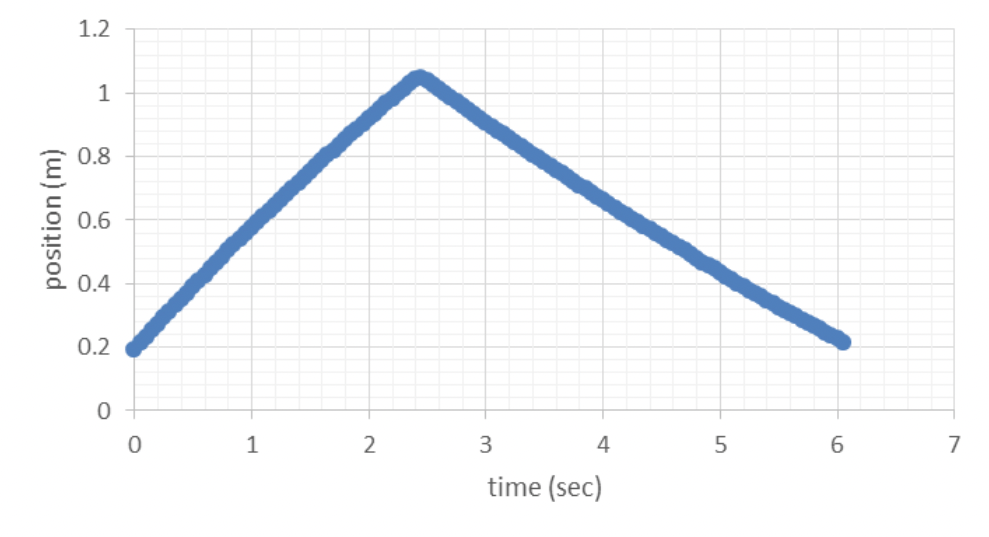
\includegraphics[width=\linewidth]{graph_1.png}
    \label{fig:graph1}
  \end{figure}

  \subsubsection{Graph analysis}
  Graph one describes the position vs. time graph of a collision.
  The graph itself directly depicts that the object's position from the sensor increases, then at
  $t\approx2.4s$ it's position begins decreasing. The derivative of a position vs. time graph gives the velocity. 
  From the slope of the graph, one can conclude that the velocity over the interval $t\epsilon[0s, 2.4s)$
  is constant and positive. Then from $t \epsilon (2.4s, 6s]$ the velocity becomes negative. With this 
  information, one can deduce the object of interest was given an initial velocity and began moving
  in the positive direction, then it encountered a barricade and reversed direction, continuing the same
  magnitude of velocity.\\
  $$\forall \, t \in [0s, 2.4s); \, v(t) = \frac{d}{dt}[s(t)] \approx 0.35m/s$$
  $$\forall \, t \in [0s, 2.4s); \, v(t) = \frac{d}{dt}[s(t)] \approx -0.35m/s$$


  \subsubsection{Setup}
  The equipment setup we choose to recreate Graph 1 consisted of a level track with a magnetic 
  bumper mounted $60cm$ from the \emph{PASCO Motion Sensor II}. We pushed and released the cart towards the bumper 
  and used the \emph{PASCO Universal 850 Interface} to track the motion using sonar. We consider 
  friction and drag negligible.\\


  
  %%%%%%%%%%%%%%%%%%%%% GRAPH 2 %%%%%%%%%%%%%%%%%%%%%
  \subsection{Graph 2}

  % Centered figure in text location
  \begin{figure}[H] % H makes the figure insert at the position in the document
    \centering 
    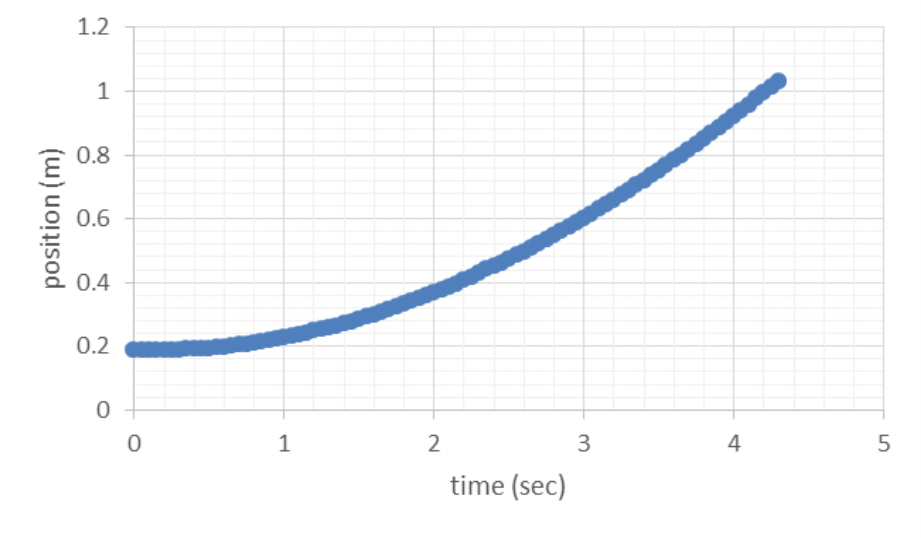
\includegraphics[width=\linewidth]{graph_2.png}
    \label{fig:graph1}
  \end{figure}

  \large{Graph discription:}\\
  \noindent{Graph 2 depicts an object speeding up at a constant rate. We know this because the
  object's position is increasing and the velocity is positive and increasing.}\\
  \large{Setup:}\\
  Our setup consisted of a track at an downward incline. We released the cart from the 
  top of the track and let it slide to the bottom. We consider friction and drag negligible.\\

  \large{Graph 3:}\\
  \large{Graph discription:}\\
  \noindent{Graph 3 depicts an object in freefall that hits the ground and stays there. We know this because the
  object's position starts from an increased height}\\
  \large{Setup:}\\
  Our setup consisted of a the sensor positioned updward. We dropped a large beach ball.\\

  \large{Graph 4:}\\
  \large{Graph discription:}\\
  \noindent{Graph 4 depicts an object moving down an incline. It comes in contact with somethinhg at the bottom and changes direction. As it changes direction it slows down. Then at $t=2.6s$ its velocity becomes negaiive but the acceleration staus positive where it is slowing down}\\
  \large{Setup:}\\
  Our setup consisted of a the sensor positioned at the biotton of an incline plane. We released the cart from the top 


  \large{Graph 5:}\\
  \large{Graph discription:}\\
  \noindent{Graph 5 depicts an object that starts from rest then is that ts pushed then slows to a stop. 
  We know this because the graph depicts the initial velocity as 0m/s, then the velocity rapidluy increases and the acceleration is posiyive. It the acceleratyion goes to zero and he velocity is constant}\\
  \large{Setup:}\\
  Our setup consisted a flat plane and w pushed the cart away from the sensor

  \large{Graph 6:}\\
  \large{Graph discription:}\\
  \noindent{Graph 6 depicts an object which is pushed and released up a hill. Eventually gravity slows it down and it 
  returns down the hill}\\
  \large{Setup:}\\
  Our setup consisted of a incline plane. We gave the cart a push and let it go up the hill then return down

  \large{Graph 6:}\\
  \large{Graph discription:}\\
  Graph 6 depicts an object moving up and swown on a spring.\\
  \large{Setup:}\\
  Our setup consisted of an downward incline. The bumper was positioned $60cm$ away from the sensor.  








  % \centerline{\textbf{Graph 1}}\\
  % % Any kind of straight lines, calculate a slope. D
  % \textbf{Graph 2}\\
  % \textbf{Graph 3}\\
  % \textbf{Graph 4}\\
  % \textbf{Graph 5}\\
  % \textbf{Graph 6}\\
  % \textbf{Graph 7}\\

  % \centerline{}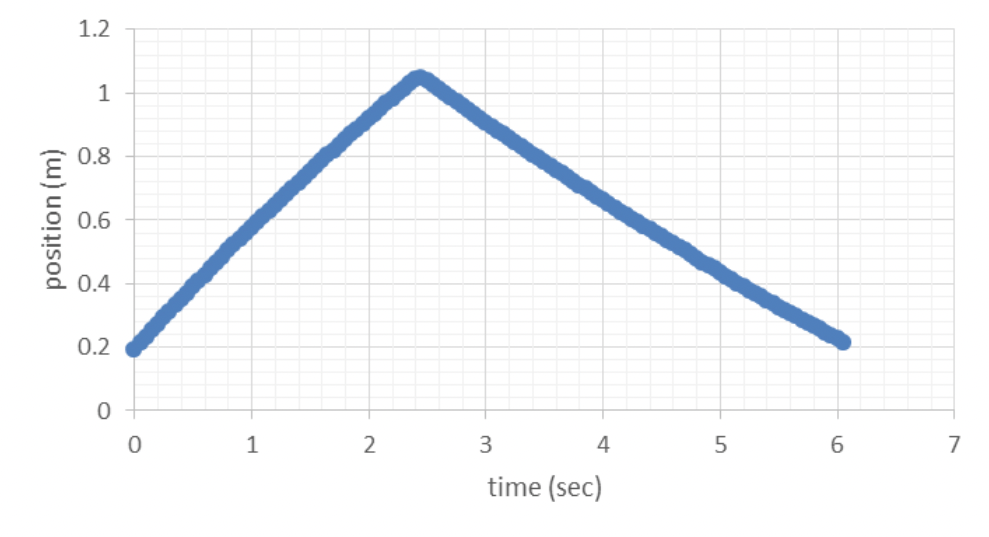
\includegraphics{graph_1.png}}

\end{document}

